\chapter{因果结构}\label{chpt:causal}


正则

\begin{definition}[因果线]
     若曲线 $\gamma$ 上任意点切矢是指向未来的类时或类光矢量(含零元),该线就成为了指向未来因果线(future directed causal curve).其他定义类似.
\end{definition}
因果线之所以要包含类光情况,是因为因果关系亦可按光速传递并影响,比如在光缆中传递的信号.然而相对论限制告诉我们,要想借助具有质量的载体传递信息,速度就是小于光速的.
\begin{definition}[未来]
    时空点 $p$ 的时序未来(chronological future)定义为集合 $I^+(p)$,其元素 $q$ 满足:存在从$p$ 到 $q$ 的类时世界线.因果未来(causal future) $J^+(p)$ 只需再包括类光情况(含零元).相应的过去集合符号将 $+$ 改为 $-$.
\end{definition}
\begin{definition}[因果菱形]
    从 $p$ 到 $q$ 的因果菱形(causal diamond)或因果核 $D_p^q$ 是指 $J^+(p)\cap J^-(q)$.
\end{definition}

\begin{theorem}
    从 $p$ 到 $q$ 的所有指向未来因果线在时空中扫出的区域含于 $D_p^q$ .
\end{theorem}
\begin{proof}
    假设 $p,q$ 间存在并不完全落在 $D_p^q$中的因果线,不落在 $D_p^q$ 的点仍同 $p,q$ 间存在因果线,因而又属于 $J^+(p),J^-(q)$,矛盾.
\end{proof}
要想完全仅用可导曲线扫出 $D_p^q$ 是不可能的,因为很明显 $\partial D_p^q$ 就是不可导的,但它确实似乎是一条物理经验上“允许”的路径,尽管这样拐角处加速度得“无穷大”才可使速度突变\footnote{这种“碰撞”理想模型的加速度符合 \textit{Dirac $\delta$ 分布}.}.在现实情况中,实际刚体的分子微扰将反而使近似宏观现象可导,甚至是光滑的,因而很多情况下可直接假定模型具有极其优良的性质,只不过这不太符合数学家的癖好.少数情况,如讨论时空奇点时,则有必要讨论许多极端情形.下面给出 Penrose 所发明的一个有用概念:
\begin{definition}[旅程]
    一个旅程(trip)或旅途就是一条“分段类时测地线”,即由有限段的测地世界线连接而成的连续曲线.这样连接点处允许不可导.“分段因果测地线”称为因果旅程.
\end{definition}
可以证明,如果用分段的类时测地线替代原来的类时线,给出的 $I^+(p),J^+(p)$ 等概念仍是等价的\footnote{早期证明由 Penrose 给出,一旦在补充少量知识后,证明将非常通俗.}.此后要想讨论一般的类时世界线,就可直接替代为旅程(指向未来因果线对应替换为因果旅程),这将大大地简化各类话题的数学细节.总之,可导曲线只能扫出 $D_p^q$ 的内部开集,替换为旅程概念后,$D_p^q$ 就可完全扫出.

\section{时空}


参考系要求时空至少在某一开域 $U$ 的时间定向性:

规定参考系矢量场指向未来

取号差 $+2$。取一 Lorentz 流形 $(M,\bm g)$ 及其切丛 $TM$。对某点 $p\in M$,若矢量 $\bm v$ 的模方 $\bm v \cdot \bm v$ 为正、负或零,那就分别称为\textbf{类空}、\textbf{类时}或\textbf{类光}矢量。所有类光矢量之集 $C_N$ 构成 $T_p M$ 的子集,称为\textbf{光锥}。

指向未来矢量所构成的子集 $\tilde F_p\subset T_p\R^{1,3}$ 称\textbf{指向未来部分},另一部分 $\tilde P_p$ 同理称\textbf{指向过去部分}。

任一事件 $p$ 的全体非零类时和类光矢量可分为此二大类,然而无论弯曲还是平直,一点的切空间当然不受影响,因此弯曲 Lorentz 流形中任一点的非零类时、类光矢量的集合也可类似地分为两大部分。

只孤立地讨论 Lorentz 流形一点 $p$ 固然可任意指定,但在讨论全时空时,物理上有理由期望这种指定在从一个时空点到另一时空点的过渡中是连续的。

当然,并非所有 Lorentz 流形都能做到这一点:
    \begin{eg}
        考虑用圆柱面 $S^1\times\R$ 表示时空,设度规这样给定:沿着任意 $S^1$ 一圈,其上光锥将均匀地旋转 $180^\circ$。这样便无法连续地指定$\tilde F$,因为若尝试按此指定,则一定存在某母线 $\R$ 上的 $\tilde F$ 有 $180^\circ$ 的突变。不妨认为这样的 Lorentz 流形没有物理意义。
    \end{eg}
\begin{definition}
    能连续地指定未来光锥的 Lorentz 流形叫\textbf{时间可定向的}(time orientable) Lorentz 流形。
\end{definition}
\begin{theorem}
    存在连续类时矢量场的 Lorentz 流形等价于时间可定向 Lorentz 流形。
\end{theorem}
\begin{proof}
    充分性上,设 Lorentz 流形存在一个连续的类时矢量场,就可把其在每点的值所在部分指定为指向未来部分,进而使得指定是连续的。必要性证明需要其它数学知识,且可见 Penrose(1972)。
\end{proof}


注意,谈到物理上合理的时空一般还要求时间可定向条件,并认为每一时空点都已作了这样的连续指定,也就是\textit{时间定向的(time oriented)},即只要可定向,那么已规定好了的就是时间定向的。不过考虑到有时玩具模型也会在称呼上用“时空”,因此 Lorentz 流形的定义不必太苛刻。若严苛一点就是:
    \begin{definition}
        \textbf{时空}通常强调是\textbf{时间定向时空},即已做时间定向的时间可定向 Lorentz 流形。
    \end{definition}
    类时矢量场结合度规可确定出光锥,因此时间定向又可用 $C_N$ 场表示。换句话说,每一点的(未来)光锥决定了时空结构(准确说是因果结构)。一点光锥称局部的,而光锥场就称整体的。因此大尺度宇观结构需要研究其上光锥场。

    有一个重要的例子:
    \begin{eg}
        \textbf{闵氏时空}是 $(\R^4,\upeta)$(记作 $\R^{3+1}$),其中 $\R^4$ 是指在 4 维实空间基础上,赋予了通常拓扑 $\mathcal T_u$ 和最大非怪异图册 $\{(O_\alpha,\psi_\alpha)\}$ 的光滑流形;$\upeta$ 称为\textbf{闵氏度规场},其定义是:$\R^4$ 的自然坐标系 $\{x^\mu\}$(这当然是 $\{(O_\alpha,\psi_\alpha)\}$ 中的一个图)在切丛里导出的坐标基底场,应使 $\upeta$ 场的分量在 $\R^4$ 上处处等于 $\eta_{\mu\nu}$,即
        \eq{
            \upeta=\eta_{\mu\nu}\d x^\mu\otimes\d x^\nu.
        }
    \end{eg}



    排除怪异图册是为排除那些在物理上不太可能的微分结构(如怪异 $\R^4$)。通常说的平直时空是指 $\R^{3+1}$。但“平直性”$\iff$ Riemann 内禀曲率张量为零张量,因此严格来说平直时空只要求配上 $\upeta$,无关于时空背景 $M$。

\begin{definition}
    \textbf{世界线}指 $(M,g)$ 上的曲线或路径\footnote{注意,虽然狭义相对性原理限制了我们只在惯性系讨论物理,但现代理论认为狭相的研究背景就是 $\R^{3+1}$,因此可用现代几何语言讨论非惯性运动(进而非惯性系),即任意世界线。在一般的时空上更是可以谈及,且结合广义协变性,甚至是任意坐标系。毕竟坐标是对物理定律描述的冗余,类似于规范不变(但不同)。}。
\end{definition}

下面研究所谓的类时世界线。指向未来的切矢总满足 $\dv*{t}\cdot\bm e_0<0$,其实亦即 $\text dx^0/\text d t>0$,我们一般默认类时世界线上参数是这样选择的(显然能使参数单调)。准确来说,还要规定参数是均匀的,即保持切矢模长。这种参数称为仿射参数。甚至可以保证切矢归一:设 $C: I \rightarrow M$ 是类空或类时线(类光线线长总为零,不必讨论),则线上任一点 $C(t')$ 的切矢 $\dv*{t'}$ 的模长是 $t'$ 的函数。任意指定线上一点 $C\left(t_0\right)$ 作为线长测量零点,则 $[t_0,t]$ 对应曲线段的线长 $L=\int_{t_0}^t\sqrt{|g(\partial_{t'},\partial_{t'})|}\mathrm{d} t^{\prime}$ 是关于 $t$ 的函数。$L$ 本身也可充当该线的参数,称为\textit{线长参数}。由 $\mathrm{d} L=\sqrt{|g(\partial_{t'},\partial_{t'})|}\mathrm{d} t^{\prime}$ 可知,线长参数给出的切矢有单位长。

\begin{definition}
    若一段类时线的切矢均指向未来,且其参数为线长参数,则称为\textbf{类时世界线}(或\textbf{指向未来类时线})。在物理上,它的像与某个质点历程中的全部事件之集等同。
\end{definition}
\begin{definition}
    一段类时世界线的线长称为该过程\textbf{所经历的固有时}。对 $\left[\xi_{0},\xi_{1}\right]$ 中的任意 $\xi$,考虑类时世界线 $\alpha$ 从 $\alpha\left(\xi_{0}\right)$ 到 $\alpha(\xi)$ 所经历的固有时
    \eq{\tau(\xi)=\int_{\xi_{0}}^{\xi} \sqrt{-g(\partial_\zeta,\partial_\zeta)} \mathrm{d} \zeta,}
    则 $\tau={\tau}(\xi)$ 总存在逆函数 $\xi=\xi(\tau)$,所以 $\alpha$ 可用 $\tau$ 来参数化。该参数正是类时世界线的线长参数,故又称\textbf{固有时参数}。
\end{definition}
观者(其世界线类时)所配备的标准钟的读数是固有时的物理性定义,无论零点如何,任意两读数的差总是等于此过程的线长。




\section{可定向性}

\section{因果线}

\section{因果条件}



\begin{figure}[h!]\centering
    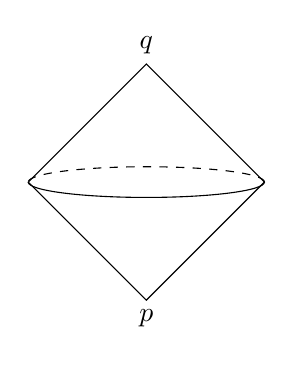
\begin{tikzpicture}[scale=1.5]
    \draw (0,1)node[above]{$q$}--(1,0)--(0,-1)node[below]{$p$}--(-1,0)--cycle;
    \draw[dashed] (1,0) arc [start angle=0, end angle=180, x radius=1, y radius=0.13];
    \draw (1,0) arc [start angle=0, end angle=-180, x radius=1, y radius=0.13];
    \end{tikzpicture}
    \caption{3 维平直时空的因果菱形。可见其形似一颗“钻石”,而其 2 维截面为“菱形”状(准确说呈平行四边形)。英语世界皆以“diamond”代之。}
\end{figure}


\section{共轭点}

\begin{wrapfigure}{l}{.3\textwidth}
    \centering
    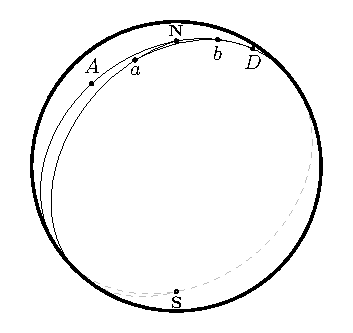
\includegraphics[width=.3\textwidth]{fig/chpt01/sphere.pdf}
    \caption{共轭点}
\end{wrapfigure}

如图,球面的南北极 $\mathbf N,\mathbf S$ 间存在无数等长测地线.从 $\mathbf S$ 出发到 $D$ 的测地线可以是 $\mathbf S A \mathbf N D$.但其长度甚至并非极小.


测地线, 其长度却并非极小, 因其非常邻近的曲线 $s b \cup \gamma$ 比它还短. 测地线 sand 的长度之所以不是极小, 关键在于线上有北极点 $n$, 它与南极点 $s$ “共轭” , 即存在从 $s$ 到 $n$ 的与测地线 $\gamma_1$ “无限邻近” 的测地线 $\gamma_2$ ( “共轭点对” 的准确定义见选读 7-6-3). 

可以证明, 测地线长度取极小值的充要条件是线上不存在共轭点对. 欧氏空间当然没有共轭点对, 因此两点之间直线(段)最短.


曲线 $s b \cup \gamma$ 在 $b$ 点不可微, 严格说应在 $b$ 点附近对它 “磨光”, 磨光后的曲线的长度与 $s b \cup \gamma$ 的长度 “要多接近有多接近”.



地线. 再讨论一般时空. 设 $C$ 是 $p, q$ 间长度极大的类时线,则由定理 3-3-6 可知它是测地线. 然而反过来却未必,因为定理 3-3-6 只保证 $p, q$ 间的类时测地线长取极值, 不保证它是极大 (当然, 由于类光曲线长度为零, 它肯定也不是极小. ). 可以证明,任意时空中类时测地线长为极大的充要条件是线上不存在共轭点对. 


 对任意时空中有类时联系的两点: (1)两点间的最长线是类时测地线; (2)两点间的类时测地线未必是最长线(对闵氏时空一定是); (3)两点间没有最短类时线.


Cauchy 发展

\section{整体双曲时空}

渐近平直时空的共性变换

引力能量非定域性

Cauchy 动力学与奇点定理

\section{Penrose 过程}

\section{能量条件}
\section{奇点定理}


类光 Raychaudhuri 方程
\section{Witten 迅捷性}
陷俘面
\section{宇宙监督假设}
\section{高-Wald 定理}


